\documentclass[12pt]{article}

\setlength\parindent{0pt}
\newcommand{\myt}[1]{\textbf{\underline{#1}}}

\usepackage{mathtools}
\usepackage{amssymb}
\usepackage{graphicx}

\title{\vspace{-15ex}Math 239 Lecture 17\vspace{-1ex}}
\date{June 15th, 2015}
\author{Graham Cooper}

\begin{document}
	\maketitle
	
	\section*{Isomorphism}
	$G_1$ is isomorphic to $G_2$ if $\exists$ a bijection $f: V(G_1) \rightarrow V(G_2)$ such that $uv \in E(G_1) \iff f(u)f(v) \in E(G_2)$.\\
	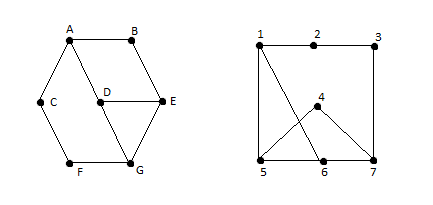
\includegraphics[scale=0.5]{isomorphic.png}
	
	8 Edges in first image, 9 edges in second. 
	
	See images on seperate page.\\
	$G_1$ and $G_2$ are not isomorphic, there exists 3 mutually adjacent vertices in $G_1$ but no such vertices exist in $G_2$.\\
	
	$G_2$ and $G_3$ are isomorpic\\
	
	\begin{tabular}{c | c c c c c c}
		v & A & B & C & D & E & F \\ \hline
		f(v) & V & III & IV & II & VI & I \\
	\end{tabular}
	
	Summary: Isomorphism is a bijection between vertices so that adjacency strcture of the edges is preserved.\\
	
	To prove 2 graphs are isomorphic, give an isomorphism.\\
	To prove 2 graphs are not ismorphic, find a structure in one graph that does not exist in the other.\\
	
	\subsection*{Spectial Graphs}
	\subsubsection*{Complete Graph}
	A complete graph is one where every pair of vertices is an edge\\
	A complete graph on n vertices is denoted $k_n$
	
	Example: \\
	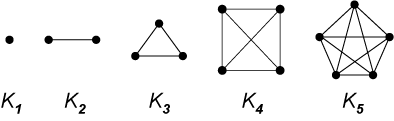
\includegraphics[scale=0.5]{completegraphs.png}\\
	
	How many edges are in $K_n$\\
	$$\frac{n(n-1)}{2} = {n \choose 2}$$
	There are ${n \choose 2}$ pairs, each forming an edge.
	
	\subsubsection*{K-regular}
	Example: \\
	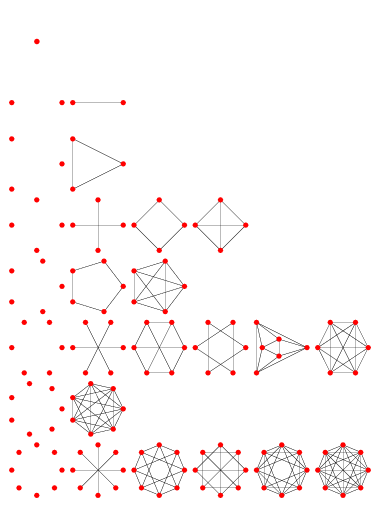
\includegraphics[scale=0.5]{k-regular.png}\\
	
	How many eges are there in a k-regular graph with n vertices?
	(Recall: Handshake Lemma $\sum deg(V) = 2|E(G)|$)\\
	The total degre is nk, so the number of edges is $\frac{nk}{2}$\\
	
	\subsubsection*{Bipartite}
	A graph G is bipartite if there exists a partition (A,B) of V(G) such that each edge in E(G) joins one vertex in A with one Vertex in B.\\
	
	Example: \\
	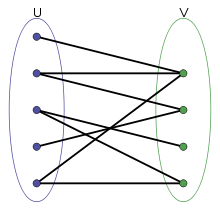
\includegraphics[scale=0.5]{bipartite.png}\\
	
	If it is bipartite then we get an edge joining 2 vertices of the same part, this is not possible so it is not bipartite. (A triangle)\\
	
	Any graph containing a griangle is not bipartate, any cycle with an odd number of vertices is not bipartite\\
	
\end{document}
